\documentclass{article}
\usepackage[utf8]{inputenc}

\usepackage{tikz}
\usetikzlibrary{matrix,arrows,decorations.pathreplacing,tikzmark,calc}
\tikzset{break/.style={fill=white, inner sep=1pt}}
\tikzset{inline/.style={column sep = 2.5em,inner sep = 1pt}}
\usetikzlibrary{arrows,positioning}

\usepackage{amsmath,amsfonts,amsthm,amssymb,thmtools,mathtools,mathrsfs,dsfont}
\usepackage{bbold}
\usepackage{graphics}
\usepackage{caption}
%\usepackage{subcaption}
\usepackage{epstopdf}
\usepackage{enumerate}
\usepackage{enumitem}
\usepackage{etex}
\usepackage{setspace}
\usepackage{chngpage}
\usepackage{soul}
\usepackage{ifthen}
\usepackage{indentfirst}
\usepackage{listings}
\usepackage{url}
\usepackage{longtable}
\usepackage{rotating}
\usepackage{float}
\usepackage{microtype}
\usepackage{lineno}
\usepackage{natbib}
\usepackage[caption = false]{subfig}
\usepackage[margin=1in]{geometry}
%\linenumbers
\allowdisplaybreaks

\usepackage[labelfont=bf]{caption}
\usepackage{multirow}



\usepackage{array}
\newcolumntype{L}[1]{>{\raggedright\let\newline\\\arraybackslash\hspace{0pt}}m{#1}}
\newcolumntype{C}[1]{>{\centering\let\newline\\\arraybackslash\hspace{0pt}}m{#1}}
\newcolumntype{R}[1]{>{\raggedleft\let\newline\\\arraybackslash\hspace{0pt}}m{#1}}


%%%%%%%%%%%%%%%%%%%%%%%%%%%% -ENVIRONMENTS-%%%%%%%%%%%%%%%%%%%%%%%%%%%%%%%%%%%%%%%%

\theoremstyle{plain}
\newtheorem{theorem}{Theorem}[section]
\newtheorem{lemma}[theorem]{Lemma}
\newtheorem{proposition}[theorem]{Proposition}
\newtheorem{corollary}[theorem]{Corollary}
\theoremstyle{definition}
\newtheorem{definition}[theorem]{Definition}
\newtheorem{example}[theorem]{Example}
\newtheorem{remark}[theorem]{Remark}
\newtheorem{algorithm}[theorem]{Algorithm}

\DeclareMathOperator*{\argmax}{arg\,max}
%\newtheorem{running example}[theorem]{Running Example}
%\newtheorem*{construction}{Construction}

%\newtheorem*{note}{Note}
%\newtheorem{conjecture}[theorem]{Conjecture}
%\newtheorem*{notation}{Notation}


\newcommand{\simplex}{\mathcal{S}}

\title{Nonlinear Incidence Caused by Phenomenological Heterogeneity in Infectious Disease Dynamics with Random Network Approaches}
\author{Author}
%\author*[1,2]{\fnm{First} \sur{Author}}\email{iauthor@gmail.com}

%\author[2,3]{\fnm{Second} \sur{Author}}\email{iiauthor@gmail.com}
%\equalcont{These authors contributed equally to this work.}

%\author[1,2]{\fnm{Third} \sur{Author}}\email{iiiauthor@gmail.com}
%\equalcont{These authors contributed equally to this work.}

%\affil*[1]{\orgdiv{Department}, \orgname{Organization}, \orgaddress{\street{Street}, \city{City}, \postcode{100190}, \state{State}, \country{Country}}}

%\affil[2]{\orgdiv{Department}, \orgname{Organization}, \orgaddress{\street{Street}, \city{City}, \postcode{10587}, \state{State}, \country{Country}}}

%\affil[3]{\orgdiv{Department}, \orgname{Organization}, \orgaddress{\street{Street}, \city{City}, \postcode{610101}, \state{State}, \country{Country}}}
\date{}


\begin{document}

\maketitle
\begin{abstract}
\bigskip
Abstract
\end{abstract}

\section{Introduction}
\label{sec: Intro}

Compartmental models with dynamics controlled by a system of ordinary differential equations, like the well-known susceptible-infectious-recovered (SIR) model discussed by Kermack \& McKendrick\cite{KermMcKe}, are commonly used when modeling disease transmission. 

\begin{figure}[htbp]
	\begin{center}
		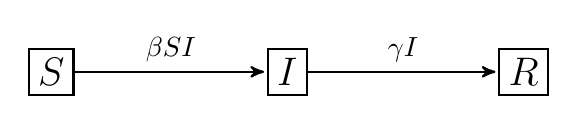
\begin{tikzpicture}[->, >=stealth',shorten >=1pt,auto, node distance=3cm, thick, main node/.style={rectangle,draw, font = \sffamily\Large\bfseries}]
			
			\node[main node] (S) {$S$};
			\node[main node] (I) [right of=S] {$I$};
			\node[main node] (R) [right of=I] {$R$};
			\draw[thick,->] (S) -- (I) node[midway,sloped,above,rotate=0] {$\beta S I$};
			
			\draw[thick,->] (I) -- (R) node[midway,sloped,above,rotate=0] {$\gamma I$};
			
		\end{tikzpicture}
	\end{center}
	\caption[Basic SIR model]{Flow diagram of a simple version of SIR model. The susceptible, infectious and recovered/removed compartments are represented by $S$, $I$ and $R$ respectively. The incidence of infection has a rate equal to the product of $S$ and $I$ times a constant per-infected transmission rate of $\beta$, which governs the flow from $S$ to $I$. The flow from $I$ to $R$ represents recovery of infectious individuals with a per capita rate $\gamma$. Figure was created using Latex Tikz Picture.}
	\label{fig: MA-SIR}
\end{figure}

These models often assumes that the population is homogeneous and fully mixed, while the contacts between individual follows the law of mass-action, such that the new infection is governed by a incidence term that is linear with respect to each involved compartment size, like the $\beta S I$ flow of the example SIR model in Figure~\ref{fig: MA-SIR}.

Such assumptions simplify the dynamic system and keep the model analysis mathematically tractable, but they are hard to associated with the heterogeneous nature of the population, where individuals could vary in different parameters that affect the transmission, like susceptibility, contact rates and infectivity.
Already back to when the model is developed (McKendrick 1939), such inconsistency drove the modelers to alternative these assumptions when fitting the data. 

To take such parametric heterogeneity into compartmental models while keep reasonable level of tractability, the common way is to divide population into limited number of groups that each have different characteristic parameter for transmission. 
Such approaches often assume that each group are homogeneous and still assumes that the population is fully mixed, so the new incidence is still governed by linear terms with respected to involved compartment size.
A important disadvantage of this approach is heterogeneity within a group cannot be incorporated with a small number of groups (Novozhilov 08), which might not align well with the variation in individuals.
Also, the fully mixing assumption limits the ability to consider heterogeneity in contact patterns.

\textbf{Another approach is to consider parametric heterogeneity of population in a more phenomenological way, such that the incidence is governed by some non-linear, functional format of the current state of the dynamic system. }

Early approaches (literature): the nonlinear incidence are raised to fit data, but lack of solid mechanistic understanding.

Later, Novozhilov \& DwyerParsons approaches provide more mechanistic explanation to some nonlinear incidence term like $I S^p$ but focus only on parametric heterogeneity of susceptibility.
Some attempts are made for consider infectivity and connectivity(identical in and out degree), but with limitations.
Very rare to discuss connectivity with locality i.e. stable social structure. 

Network and random network approach: from Pastor-Satorras, to Newman, to MSV, to Zhao-Magpantay

Here in this manuscript, we investigate phenomenological heterogeneity of susceptibility, connectivity and locality together under the MSV random network framework to reveal new perspective and understanding of nonlinear incidence.



\subsection{SubSection}
\label{sec: sub1}
\textit{Treponema pallidum} subspecies pallidum\cite{DushoffEtAl:2004,BansalMeyers:2012}.

Itemize
\begin{itemize}
\item a

\item b

\item c
	\begin{itemize}

	\item (1)

	\item (2)

\end{itemize} 

In practice, diagnoses of early versus late latent stages are determined based on serological testing and clinical input.

\item d

\end{itemize}

\section{Data}
\label{sec: data}


\section{Model Setup}
\label{sec: model}

Enumerate
\begin{enumerate}
\item [(H1)] Assumption
\end{enumerate}

\subsection{Subsection}
\label{sec: sub 2}


Equation
\begin{equation}
    \mathbb{P}(K=k) \propto k^{-\alpha}
    \label{eqn: power law}
\end{equation} 

package \verb#fit_power_law# function from the \verb#igraph# R package

Eqref: \eqref{eqn: power law}.

Class Eqns
\begin{equation}
\label{eqn: CM ODE}
    \begin{cases}
        S(t) & = G_p(\theta(t)) \\
        I(t) & = 1-S(t)-R(t) \\
        \dot{R}(t) & = \gamma I(t) \\
        \dot{\theta}(t) & = -\beta \theta +\beta \frac{G'_p(\theta)}{G'_p(1)}+\gamma (1-\theta)
    \end{cases} 
\end{equation}



\section{Comparing the network-SIR and MA-SIR models}
\label{sec: MA compare}


\section{Conclusions}
\label{sec: Conclusion}


\section*{Acknowledgments}
We thank XX for his help with the literature review. 

\section*{Funding Statement}
Funding

\newpage
\bibliographystyle{unsrt}
\bibliography{Bibliography}

\newpage
%% Supplementary materials
%% Reset all counters and include S at the beginning of 
\setcounter{equation}{0}
\setcounter{figure}{0}
\setcounter{table}{0}
\setcounter{section}{0}
\setcounter{page}{1}
\makeatletter
\renewcommand{\theequation}{S\arabic{equation}}
\renewcommand{\thefigure}{S\arabic{figure}}
\renewcommand{\thetable}{S\arabic{table}}
\renewcommand{\thesection}{S\arabic{section}}
%\renewcommand{\bibnumfmt}[1]{[S#1]}
%\renewcommand{\citenumfont}[1]{S#1}

\begin{center}
{\huge \sc   Supplementary Information}
\end{center}

\section{Section}
\label{sec: sup 1}


\begin{center}
    \begin{table}[htbp]
    \centering
\caption{Table Exp}
    \label{table: example}
        \begin{tabular}{|C{1.0in}|C{1.0in}|C{0.8in}|C{0.8in}|C{0.8in}|}
            \hline
            \multicolumn{3}{|c|}{Age Groups} & \multicolumn{2}{c|}{Scaling Parameters}
            \\
            \hline
            Age range & Risk Level & Proportion & Symbol & Value
            \\
            \hline
            $[18,20)$ & Medium & 1.25\% & $a_1$ & 0.150
            \\
            \hline
            $[20,30)$ & High & 26.97\% & $a_2$ & 0.250
            \\
            \hline
            $[30,40)$ & Medium & 40.66\% & $a_3$ & 0.150
            \\
            \hline
            $[40,50)$ & Low-Medium & 21.16\% & $a_4$ & 0.050
            \\
            \hline
            $[50,\infty)$ & Low & 9.96\% & $a_5$ & 0.025
            \\
            \hline
        \end{tabular}
    \end{table}
\end{center}



\begin{center}
    \begin{table}[htbp]
    \centering
\caption{Complex Table Example}
\label{table: Complex}
\begin{tabular}{|C{2.4in}|C{0.4in}|C{0.9in}|C{0.7in}|C{0.7in}|}
            \hline
            \multicolumn{3}{|c|}{Risk Factor Groups} & \multicolumn{2}{c|}{Scaling Parameters}
            \\
            \hline
            Factor Description & Count & Group & Symbol & Value 
            \\
            \hline
            Anonymous Sex & 42 & \multirow{3}{0.7in}{\centering Anonymous Sex} & \multirow{3}{*}{$r_1$} & \multirow{3}{*}{$0.6$} 
            \\
            \cline{1-2}
            Met contact through internet & 5 & & &
            \\
            \cline{1-2}
            Bath house & 1 &  &  &
            \\
            \hline
            Repeat STI & 55 & \multirow{5}{0.7in}{\centering STI} & \multirow{5}{*}{$r_2$} & \multirow{5}{*}{$0.2$} 
            \\
            \cline{1-2}
            Co-Infection with other STI & 10 & & &
            \\
            \cline{1-2}
            HIV Status & 5 &  &  &
            \\
            \cline{1-2}
            PrEP for HIV & 4 &  &  &
            \\
            \cline{1-2}
            HIV positive contact & 1 &  &  &
            \\
            \hline
            Pregnant & 16 & \multirow{8}{0.7in}{\centering Pregnancy Related} & \multirow{8}{*}{$r_3$} & \multirow{8}{*}{$0.0$} 
            \\
            \cline{1-2}
            Tested during first Trimester & 4 & & &
            \\
            \cline{1-2}
            Treated $>4$ weeks prior to delivery  & 2 &  &  &
            \\
            \cline{1-2}
            Received prenatal care & 2 &  &  &
            \\
            \cline{1-2}
            Tested at delivery & 1 &  &  &
            \\
            \cline{1-2}
            Tested at 28-32 Weeks & 1 &  &  &  
            \\
            \cline{1-2}
            Tested $>4$ weeks prior to delivery & 1 &  &  &  
            \\
            \hline
            Correctional facility & 20 & \multirow{1}{0.7in}{\centering Prison} & \multirow{1}{*}{$r_4$} & \multirow{1}{*}{$0.2$} 
            \\
            \hline
            Under-housed/Homeless & 28 & \multirow{1}{0.7in}{\centering SES} & \multirow{1}{*}{$r_5$} & \multirow{1}{*}{$0.0$} 
            \\
            \hline
            No condom used & 55 & \multirow{4}{0.7in}{\centering Sex Behavior} & \multirow{4}{*}{$r_6$} & \multirow{4}{*}{$0.0$}
            \\
            \cline{1-2}
            More than one sex contacts & 22 &  &  & 
            \\
            \cline{1-2}
            Shared sex toys & 1 &  &  & 
            \\
            \cline{1-2}
            New sex contact in past 2 months & 23 &  &  & 
            \\
            \hline
            Sex trade worker & 11 & \multirow{2}{0.7in}{\centering Sex Trade} & \multirow{2}{*}{$r_7$} & \multirow{2}{*}{$1.0$} 
            \\
            \cline{1-2}
            Sex with sex trade worker & 6 &  &  & 
            \\
            \hline
            Sex with same sex & 45 & \multirow{1}{0.7in}{\centering Same Sex} & \multirow{1}{*}{$r_8$} & \multirow{1}{*}{$0.6$} 
            \\
            \hline
            Injection drug use & 38 & \multirow{6}{0.7in}{\centering Substance} & \multirow{6}{*}{$r_9$} & \multirow{6}{*}{$0.3$} 
            \\
            \cline{1-2}
            Inhalation drug use & 43 &  &  & 
            \\
            \cline{1-2}
            Judgement impaired by alcohol/drugs & 8 &  &  & 
            \\
            \cline{1-2}
            Shared other drug equipment & 6 &  &  & 
            \\
            \cline{1-2}
            Sex for drugs/shelter/food & 3 &  &  & 
            \\
            \cline{1-2}
            Shared needles & 2 &  &  & 
            \\
            \hline
            Tattoo and piercing & 5 & \multirow{5}{0.7in}{\centering Unknown} & \multirow{5}{*}{$r_{10}$} & \multirow{5}{*}{$0.0$} 
            \\
            \cline{1-2}
            Travel outside province & 4 &  &  &
            \\
            \cline{1-2}
            Other social venue & 1 &  &  & 
            \\
            \cline{1-2}
            Unknown & 248 &  &  & 
            \\
            \cline{1-2}
            Other & 7 &  &  & 
            \\
            \hline
        \end{tabular}
    \end{table}
\end{center}

%\begin{figure}[htbp]
%    \begin{center}
%        \includegraphics[width=0.9\textwidth]{Images/plotsMSV.png}
%    \end{center}
    %\caption[Example Plot}
%    \label{fig: Exp}
%\end{figure}

\section{Section}
\label{sec: sup 2}

%\begin{figure}[htbp]
%    \centering
%    \begin{subfigure}[b]{0.30\textwidth}
%         \centering
%         \includegraphics[width=\textwidth]{Images/plotsMSV.png}
%         \caption{subplot1}
%    \end{subfigure}
%    \begin{subfigure}[b]{0.31\textwidth}
%         \centering
%         \includegraphics[width=\textwidth]{Images/plotsMSV.png}
%         \caption{subplot2}
%    \end{subfigure}
%    \begin{subfigure}[b]{0.33\textwidth}
%         \centering
%         \includegraphics[width=\textwidth]{Images/plotsMSV.png}
%         \caption{subplot3}
%    \end{subfigure}
%    \caption{Multi-plot}
%    \label{fig: multi}
%\end{figure}

\section{Section}
\label{sec: sup 3}
%literature~\cite{LiljerosEtAl:2003, LiljerosEtAl:2001, AnneEtAl:2004} and our data.

\section{Section}
\label{sec: sup 4}


\end{document}
